%
% Latest revision 13 Sep 2014
%
\documentclass[pdf,ps2pdf,12pt]{smemo}
\usepackage{epsfig}
\usepackage[FIGBOTCAP,normal,bf,tight]{subfigure}

% ---------------------------------------------------------------------- %
% Start the document
%
\begin{document}
    \begin{memo}

    % ---------------------------------------------------------------------- %
    % Header information
    %

    % If different from today's; or use \nodate to suppress date
    \date{}

    % if to one person, put their name here
    % e.g. \to{H. S. Granger, Org. 0001, MS-9999}
    % otherwise use \to{Distribution} and include distribution list at end
    \to{Distribution}

    % For running head, if heading on following pages is not Addressee
    %\headtext{}

    % Who is this memo from; e.g., \from{J. E. Smith, Org. 0002, MS-0001}
    \from{Bill Spotz, Org 1446; Dena Vigil, Org 1441}

    % Fill in a subject
    \subject{How to Document \texttt{Teuchos::ParameterList}s with collapsable HTML}



    % ---------------------------------------------------------------------- %
    % Main text of memo begins here
    %

\section{Introduction}
\label{sec:intro}

One of the most important categories of information needed by users of
Trilinos packages or applications built with Trilinos, is valid
options for \texttt{Teuchos::ParameterList}s.  This category includes
valid parameter names, valid parameter types, valid parameter ranges
or enumerated values, and valid parameter descriptions.
\texttt{Teuchos::ParameterList}s allow for nested parameter lists, and
high-level packages or applications can end up accessing extremely
long lists of parameters, many of which are not of immediate interest
to the user.  This necessitates a user-friendly and visually appealing
method of documenting \texttt{Teuchos::ParameterList}s.  Such a method
has been developed, along with the infrastructure to support it, and
this memo provides instructions for developers who wish to use it.

Reference manual style documentation of Trilinos packages is typically
produced using Doxygen.  Doxygen can produce documentation in many
output forms, including PDF, PS, and HTML.  The documentation method
discussed here is appropriate only for HTML, as it takes advantage of
dynamic collapsible text, allowing the user to hide large chunks of
information that is not of immediate interest.

    %
    % We should put an example of what a documented ParameterList looks like here
    %

Inserting this type of content into Doxygen-generated HTML is
non-trivial, but most of the steps have been automated for the
developer's convenience.  After following the steps outlined in this
memo, you should be able to insert dynamic, collapsible documentation
of your \texttt{Teuchos::ParameterList}s inside your package's Doxygen
documentation.

\section{Examples of Documented \texttt{Teuchos::ParameterList}s}
\label{sec:examples}

The infrastructure developed for documenting
\texttt{Teuchos::ParameterList}s covers many different types of
parameters and many different types of validators.  We include here a
small sampling of what these elements look like in a web browser when
rendered using this infrastructure.

\begin{figure}[h]
  \begin{centering}
    \scalebox{0.7}{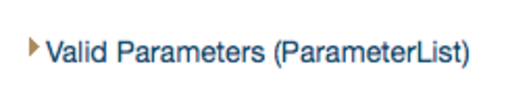
\includegraphics{ClosedTopLevelParameterList}}
    \caption{\label{fig:closed_top} A top-level ParameterList, closed}
  \end{centering}
\end{figure}

Figure~\ref{fig:closed_top} shows a top-level
\texttt{Teuchos::ParameterList} in a closed state, that is to say, all
of its content is hidden.  This is how your
\texttt{Teuchos::ParameterList} documentation will first appear in a
browser.  Clicking the text has the effect of opening the first level
of its content, shown in Figure~\ref{fig:open_top}.

\begin{figure}[h]
  \begin{centering}
    \scalebox{0.7}{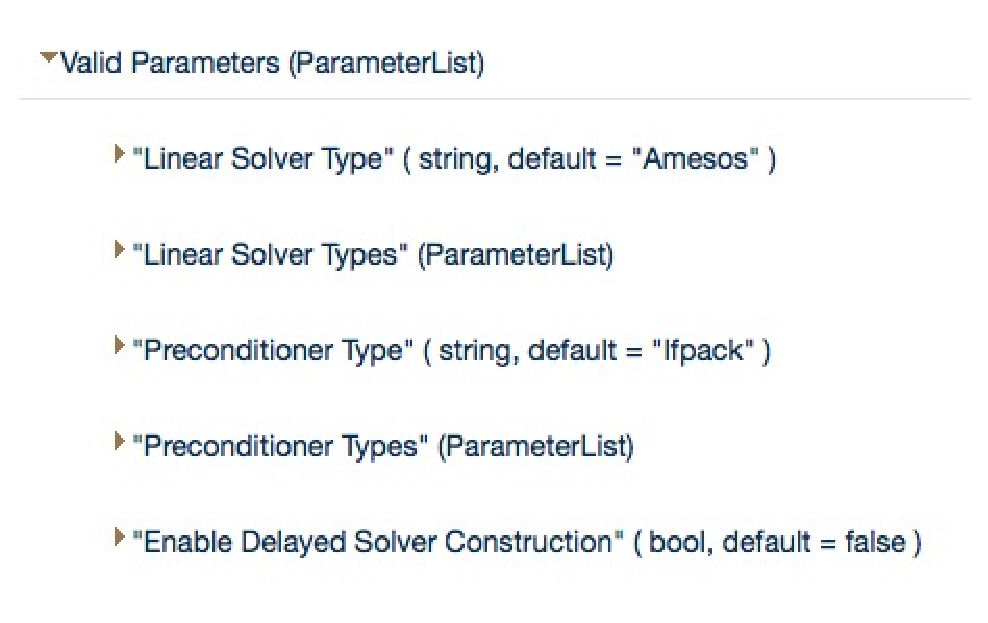
\includegraphics{OpenTopLevelParameterList}}
    \caption{\label{fig:open_top} A top-level ParameterList, open}
  \end{centering}
\end{figure}

In this case, the top-level \texttt{Teuchos::ParameterList} contains
five parameters: two string parameters, two
\texttt{Teuchos::ParameterList} sub-lists, and one boolean parameter.
Each of these parameters can be clicked to reveal more content.

\begin{figure}[h]
  \begin{centering}
    \scalebox{0.7}{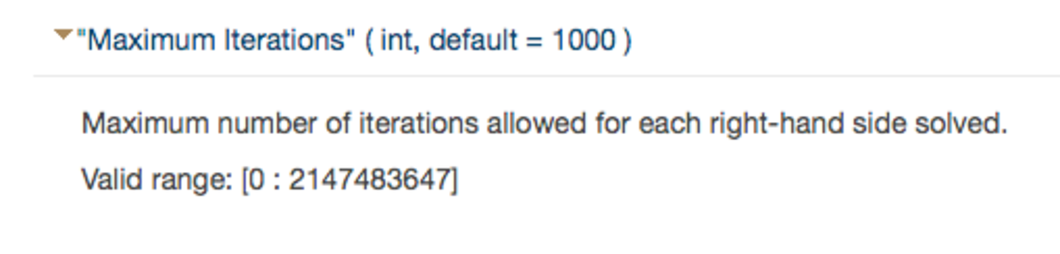
\includegraphics{OpenIntegerParameterWithValidator}}
    \caption{\label{fig:open_integer} Documentation of an integer
      parameter with validator, open}
  \end{centering}
\end{figure}

In its closed state, a parameter will generally display its name in
quotes, and in parentheses, it will display its type and default
value.  When opened, a parameter will generally display its
documentation string and validator.  Figure~\ref{fig:open_integer}
shows an integer parameter that has been clicked open to reveal a
description and the valid range of values for that parameter.

The rendering of validators can be more complicated, depending on the
validator.  Figure~\ref{fig:open_string} shows a string parameter in
an open state, with an enumerated string validator. Such a validator
provides a finite set of valid string values, and also provides a
description of each valid value.  These values and descriptions are
rendered in a table under the description of the parameter itself.

\begin{figure}[h]
  \begin{centering}
    \scalebox{0.7}{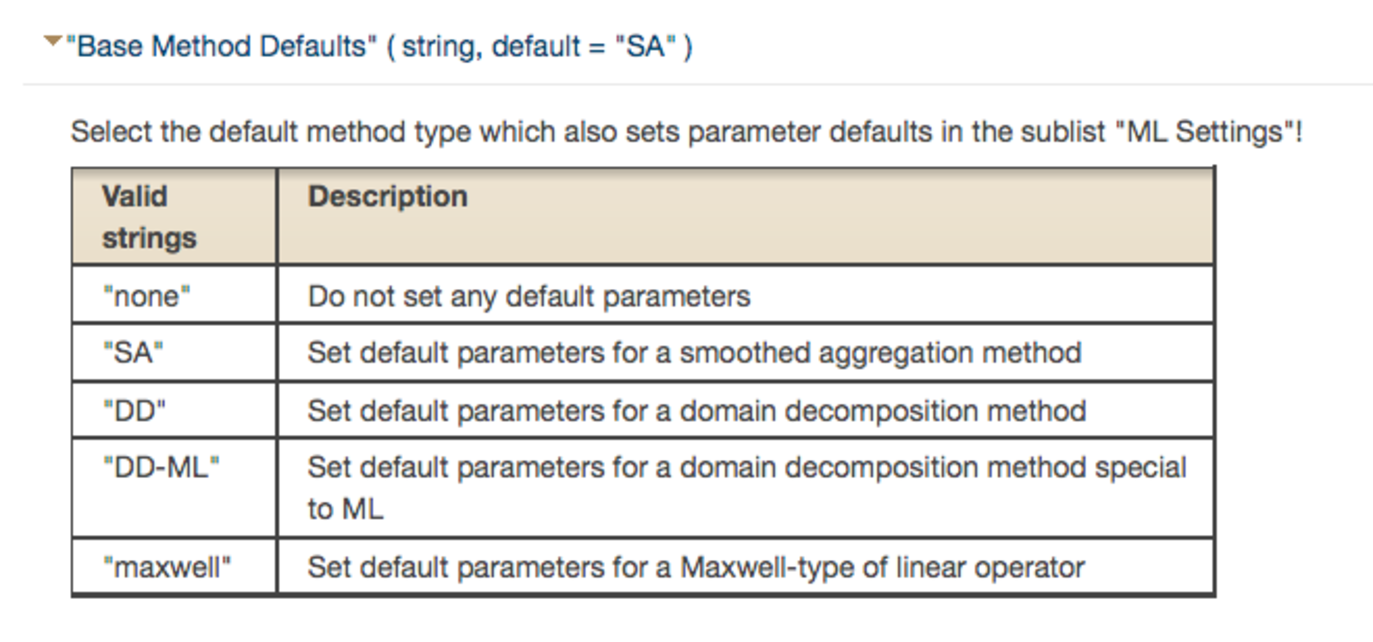
\includegraphics{OpenStringParameterWithValidator}}
    \caption{\label{fig:open_string} Documentation of a string
      parameter with validator, open}
  \end{centering}
\end{figure}

\section{Steps}
\label{sec:steps}

The high-level set of steps for documenting
\texttt{Teuchos::ParameterList}s inside a package's Doxygen
documentation is as follows:

\begin{enumerate}

\item Write a method or function within your package that returns a
  \emph{validated} \texttt{Teuchos::Pa\-ra\-me\-ter\-List} for each
  \texttt{Teuchos::ParameterList} you wish to document.

\item Copy required files from
  \texttt{Trilinos/doc/DocumentingParameterLists} to your package
  directory to enable the HTML and XML infrastructure.

\item Add (a) short executable(s) to your package build system that
  constructs this (these) validated \texttt{Teuchos::ParameterList}(s)
  and writes it (them) to (an) XML file(s).

\item Tell the Trilinos documentation build system that your package
  can generate an XML description of a validated
  \texttt{Teuchos::ParameterList} by adding your package name to the
  file \texttt{Trilinos/doc/DocumentingParameterLists/Packages.txt}.

\item Add a Doxygen directive to your source file(s) to activate the
  documentation.

\end{enumerate}

\section{Detailed Description}
\label{sec:description}

Each of the aforementioned steps require a more detailed explanation.

\begin{enumerate}

\item \textbf{Develop validated \texttt{Teuchos::ParameterList}(s).}
  The recommended approach for this is to have your class inherit from
  \texttt{Teuchos::ParameterListAcceptor} and implement the virtual
  method \texttt{getValidParameters()}.  Good subclasses of this base
  class follow the ``separate construction and just-in-time
  initialization'' idioms~\cite{TeuchosMemMgt}.  This allows a user to
  construct an instance of your class, obtain a default, validated
  \texttt{Teuchos::RCP< const Teuchos::ParameterList >}, copy and
  modify that \texttt{ParameterList}, and then use the modified
  \texttt{ParameterList} to initialize the instance.

  Of course, some (many?) classes are not designed this way, and would
  require significant refactoring to adopt this design, and might
  require breaking backward compatibility if they did.  In these
  cases, the design approach is completely up to the package
  developers.  For consistency, \texttt{getValidParameters()} is a
  good method or function name to use.

  The returned \texttt{Teuchos::RCP< const Teuchos::ParameterList >}
  should be as complete as possible.  This means a
  \texttt{Teuchos::ParameterList} in which each
  \texttt{Teuchos::Pa\-ra\-met\-er\-En\-try} is given a documentation
  string and a
  \texttt{Teuchos::Pa\-ra\-me\-ter\-En\-try\-Val\-i\-da\-tor}. This
  usually constitutes the lion's share of the effort a developer must
  exert in order to obtain useful documentation for a
  \texttt{Teuchos::ParameterList}.  But the effort is usually
  worthwhile, as a valid \texttt{Teuchos::ParameterList} also provides
  a convenient means of checking an input
  \texttt{Teuchos::ParameterList} provided by a user.

\item \textbf{Copy required files to your package.} By convention, the
  source file(s) for the executable(s) that can generate XML files
  describing your validated \texttt{Teuchos::Pa\-ra\-me\-ter\-List}(s)
  will be kept in the \texttt{doc/parameterList} directory of your
  package. This will require additional \texttt{CMakeLists.txt} files
  to augment the build system to include the new executables to be
  built. Much of this can be put in place by executing the following
  in the shell:

 \begin{verbatim}
  $ cd Trilinos/doc/DocumentingParameterLists
  $ cp -r doc/* ../../packages/<package>/doc
 \end{verbatim}

  where \texttt{<package>} is the name of your package. This assumes
  that the directory \texttt{Trilinos/packages/<package>/doc} already
  exists, which is typically the case for most Trilinos packages.  It
  also assumes that there is not already a \texttt{CMakeLists.txt}
  file in that directory.

  Finally, the \texttt{Trilinos/packages/<package>/CMakeLists.txt}
  file will have to be modified to include an
  \texttt{ADD\_SUBDIRECTORY(doc)} macro call to include the new
  infrastructure in the existing build system.

\item \textbf{Add executable(s) to generate XML file(s).} The copy
  (\texttt{cp}) command in the previous step will create a file
  \texttt{Trilinos/packages/<package>/doc/parameter\-List/\-create\-Valid\-Parameter\-List.cpp}.
  This is a template that can be easily modified to obtain a valid
  \texttt{Teuchos::ParameterList} via the method developed in Step 1,
  and write that \texttt{ParameterList} as an XML file.

  Many packages will need to support multiple
  \texttt{Teuchos::ParameterList}s.  Note that each valid
  \texttt{Teuchos::ParameterList} must have its own XML file.  This
  could be handled by having one executable write all of the XML files
  each time it is run; or by having one executable write only one XML
  file each time it is run, controlled by a command-line option; or by
  having multiple executables, each one of which writes one XML
  file. The approach is entirely up to the developers.  Whatever
  approach is chosen must be reflected in the \texttt{CMakeLists.txt}
  file in the same directory. For example, multiple executables will
  require multiple \texttt{TRIBITS\_ADD\_EXECUTABLE()} macro calls and
  corresponding \texttt{TRIBITS\_ADD\_TEST()} macro calls.  A single
  executable with different command line options will require a single
  \texttt{TRIBITS\_ADD\_EXECUTABLE()} macro call and multiple
  \texttt{TRIBITS\_ADD\_TEST()} macro calls.

  By convention, each executable must have the string
  ``\texttt{ValidParam}'' in its name.  This is because the
  documentation build system will run

 \begin{verbatim}
  ctest -R ValidParam
 \end{verbatim}

  in order to generate all of the XML files (the \texttt{-R} option
  says to only run those tests whose name matches the given regular
  expression).

\item \textbf{Add your package name to \texttt{Packages.txt}.} Simply
  modify file
  \texttt{Trilinos/\-doc/\-Documenting\-Parameter\-Lists/\-Packages.txt}
  to include your package, one package name per line.  Use the
  capitalized form of the package name, specifically the form that is
  valid for

 \begin{verbatim}
   cmake -D Trilinos_ENABLE_<package>:BOOL=ON \
         -D <package>_ENABLE_TESTS:BOOL=ON
 \end{verbatim}

  The packages listed in this file will tell the Trilinos
  documentation build system to enable your package and all of its
  optional packages when configuring and building the executables that
  write the XML files.

\item \textbf{Add Doxygen directive(s) to your source file(s).} The
  Trilinos documentation build system will automatically move the
  generated XML files to where they can be found by the generated
  Doxygen HTML files.  This is enabled in part by the python script
  \texttt{copy\_xml\_to\_src\_html.py}, which was copied to your
  \texttt{doc} directory in step 2 of sections~\ref{sec:steps}
  and~\ref{sec:description}.

  The last piece that is needed is one or more directives in the
  Doxygen comments of your source code to tell Doxygen where the
  collapsible \texttt{Teuchos::ParameterList} documentation should
  go. Typically, this would be in the section of code where arguments,
  specifically a \texttt{Teuchos::ParameterList} argument, is
  documented. The final Doxygen comment should look something like
  this for each XML file generated:

 \footnotesize
 \begin{verbatim}
    /** \brief Constructor with ParameterList
     * 
     * \param plist [in] ParameterList with construction information
     *   \htmlonly
     *   <iframe src="<base>.xml" width="100%" scrolling="no" frameborder="0">
     *   </iframe>
     *   <hr />
     *   \endhtmlonly
     */
 \end{verbatim}
 \normalsize

 where \texttt{<base>} is the base name of the appropriate XML file.
 This name will be the appropriate XML file name chosen by the
 developer, and may be the package name or something more specific to
 the class being documented.

\end{enumerate}

\section{Testing the \texttt{ParameterList} Documentation}
\label{sec:testing}

If you want to test the documentation of your package, without
building the entire Trilinos Doxygen hierarchy, you will have to
perform a couple extra steps to get your collapsible
\texttt{Teuchos::ParameterList} documentation to render properly in a
web browser.  The steps are

 \begin{enumerate}
   \item \textbf{Build a minimal Trilinos configuration with your
       package and its optional packages.}  A seasoned Trilinos
     developer can do this using any appropriate configuration he or she
     wishes.  An alternative would be to copy
\begin{verbatim}
    Trilinos/doc/DocumentingParameterLists/do-configure
\end{verbatim}
     to your build directory.  This script takes the path to the
     Trilinos source directory as its argument (using \texttt{..} as
     the default).  Use \texttt{--help} for a more detailed
     description of the script.  This script will configure Trilinos
     to build all packages that support collapsible ParameterList
     documentation, plus all of those packages' optional packages.
     Then use \texttt{make} to build Trilinos.

    \item \textbf{Run the executable(s) that generate the
        \texttt{Teuchos::ParameterList} XML files.}  The easiest way to
      do this is to run
\begin{verbatim}
    $ ctest -R ValidParam
\end{verbatim}
      from within the build directory.

    \item \textbf{Run \texttt{build\_docs} in your
        \texttt{<package>/doc} directory.}  Doxygen documentation
      continues to be built within the source directory.  All this
      requires is
\begin{verbatim}
    $ cd Trilinos/packages/<package>/doc
    $ ./build_docs
\end{verbatim}
      where \texttt{<package>} is your package name.  This will create
      an \texttt{html} directory with the HTML version of the Doxygen
      documentation within it.

    \item \textbf{Copy the XML files from your \texttt{<package>/doc}
        directory.}  This can be done automatically by running the
      script \texttt{copy\_xml\_to\_src\_html.py}, which was copied to
      your \texttt{doc} directory in step 2 of
      sections~\ref{sec:steps} and~\ref{sec:description}.  This script
      takes the path to your build directory as its argument.

 \end{enumerate}

 You are now ready to test your \texttt{Teuchos::ParameterList}
 documentation.  Simply open \texttt{html/index.html} in your browser
 and navigate to where your \texttt{Teuchos::ParameterList}
 documentation is located.

    %
    % Main text of memo ends here
    % ---------------------------------------------------------------------- %

\bibliographystyle{plain}
\bibliography{SMemo_PListDoc}

    % ---------------------------------------------------------------------- %
    % Initials, enclosures, and keywords, if necessary
    % 
    % If initials are required; e.g., \initials{ H.P. }
    % \initials{}

    % If you have enclosures
    % \enc{}

    % Should you need keywords; e.g., \keywords{ dry erase markers }
    % \keywords{}



    % ---------------------------------------------------------------------- %
    % Distribution list
    % 
    \clearpage
    \begin{distribution}{External Distribution:}
	\normalfont
        External Trilinos package developers \\
        External Trilinos application developers
    \end{distribution}

    \begin{distribution}{Internal Distribution:}
	\normalfont
        Internal Trilinos package developers \\
        Internal Trilinos application developers
    \end{distribution}

    \end{memo}
\end{document}
